%label:"fig:HmsDiagram"
%type:"figure"
%name:"HMS diagram"
%caption:"Mirror symmetry exchanges the symplectic invariants ($A$-side) and complex invariants ($B$-side) on a pair of ``mirror'' spaces."
%parent:"art_HMSForFanos2"


    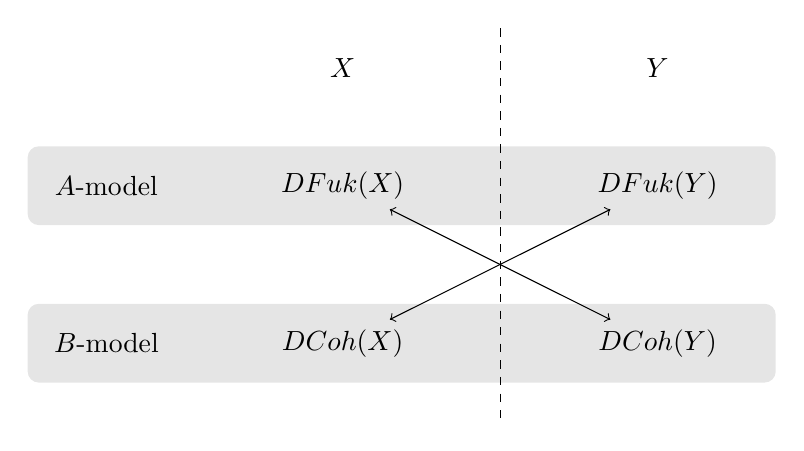
\begin{tikzpicture}

        \fill[gray!20,rounded corners]  (3.5,1) rectangle (-6,2);
        \fill[gray!20,rounded corners]  (3.5,-1) rectangle (-6,0);
        \node (v3) at (-2,1.5) {$D\text{Fuk}(X)$};
        \node (v2) at (2,1.5) {$D\text{Fuk}(Y)$};
        \node (v1) at (-2,-0.5) {$D\text{Coh}(X)$};
        \node (v4) at (2,-0.5) {$D\text{Coh}(Y)$};
        \draw[<->]  (v1) edge (v2);
        \node at (-2,3) {$X$};
        \node at (2,3) {$Y$};
        \draw[dashed] (0,3.5) -- (0,-1.5);
        \draw[<->]  (v3) edge (v4);
        
        \node at (-5,1.5) {$A$-model};
        \node at (-5,-0.5) {$B$-model};
    \end{tikzpicture}

